\subsection{Multiple Document Types Search}

\begin{frame}{Type Search}
  \begin{itemize}
    \item Desktop search
    \item Usually many document types
    \item Goal: Predicting the document type for a given query
  \end{itemize}
\end{frame}

\begin{frame}{Retrieval Model}
  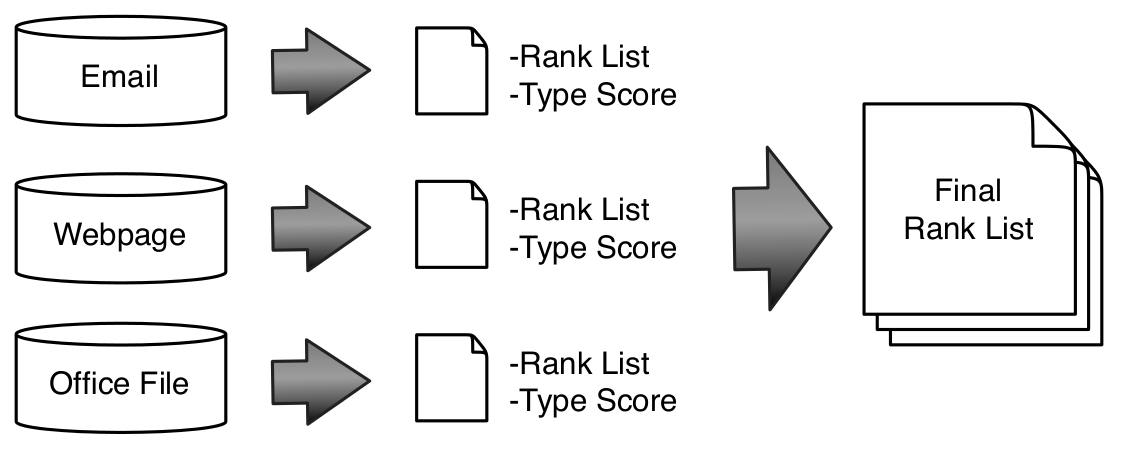
\includegraphics[width=\textwidth]{img/typeSearch.png}
\end{frame}

\begin{frame}{Retrieval Model (2)}
 Two phases
 \begin{itemize}
 \item Rank documents from each sub-collection, obtaining both a 
   rank list and a type score
 \item Merge the results
 \end{itemize}
\end{frame}

\begin{frame}{Type-specific Retrieval}
  \begin{itemize}
  \item Rank documents inside one sub-collection
  \item PRM-S: Probabilistic Retrieval Model for Semi-structured Data
  \item Use probabilities to assign a score to every document in the collection
  \end{itemize}
\end{frame}

\begin{frame}{Type Prediction}
  Methods
  \begin{itemize}
    \item Query-likelihood of Collection
      \begin{itemize}
      \item Collapse all documents in each collection into one document
      \item Use probabilities to compute score
      \end{itemize}
    \item Query-likelihood of Query Log
      \begin{itemize}
      \item For each collection obtain an aggregated list with query terms
        used for finding documents in that collection
      \item Match the input query with those lists
      \end{itemize}
    \item Match query with metadata fields
  \end{itemize}
\end{frame}

\begin{frame}{Result Merging}
  \begin{center}
    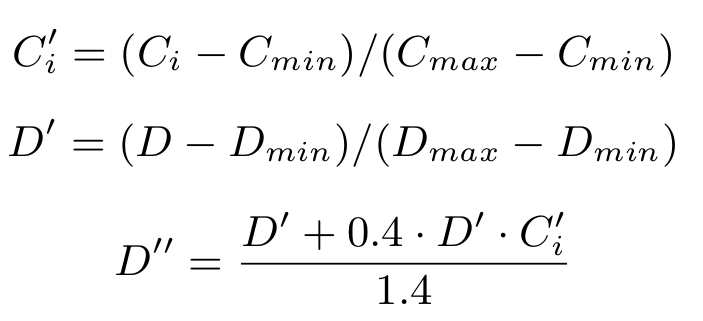
\includegraphics[width=0.6\textwidth]{img/cori.png}
  \end{center}

  \begin{itemize}
  \item CORI algorithm
  \item $D$ - document score (type-specific)
  \item $C_i$ - score for D's collection (type prediction)
  \item $C_{max}$, $C_{min}$ - maximum and minimum collection scores
  \item $D_{max}$, $D_{min}$ - maximum and minimum document scores
  \item $D^{''}$ - final document score
  \end{itemize}
\end{frame}
